\documentclass{article}

\usepackage[a4paper, total={6in, 8in}]{geometry}
\usepackage[utf8]{inputenc}
\usepackage{amsmath}
\usepackage{amssymb}
\usepackage{tabularx}
\usepackage[makeroom]{cancel}
\usepackage{arydshln}
\usepackage{graphicx}
\usepackage{fancyhdr}
\usepackage{enumitem}

\pagestyle{fancy}
\fancyhf{}
\lhead{John J Li}
\rhead{CSE205 Spring 2021 Homework 4}
\rfoot{\thepage}
\lfoot{March 2021}
\renewcommand{\headrulewidth}{0.4pt}
\renewcommand{\footrulewidth}{0.4pt}

\setlength{\parskip}{1em}
\setlength\parindent{0px}
\title{CSE205 Spring 2021 Homework 4}
\date{\today}
\author{John J Li}

\begin{document}
    \maketitle
    \thispagestyle{empty}
    \noindent\rule{\textwidth}{0.8pt}

    %###################################################################################

    \section*{Problem 1}

    Compute the maximum delay, assume every gate (gate includes the attached negation bubbles) 
    has a delay of $\Delta$. Assume only uncomplemented inputs are available and an additional gate 
    must be added to complement any input marked X’.

    \begin{center}
        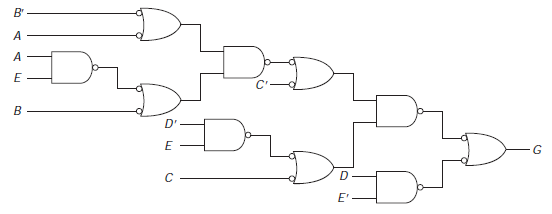
\includegraphics[width=\linewidth]{Problem_1.png}
    \end{center}

    \begin{enumerate}[label={\bfseries Solution:}, leftmargin=*]
        \item Since we can see that inputs A and E will have to 
        go through 6 logic gates and we assumed every gate has a delay of $\Delta$, the maximum delay is $6\Delta$. 
    \end{enumerate}

    %###################################################################################

    \section*{Problem 2}

    Create the truth table that belongs to the following multiplexer implementing function 
    F(A, B, C).

    \begin{center}
        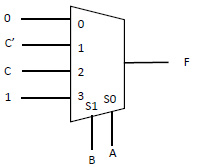
\includegraphics[scale=0.75]{Problem_2.jpg}
    \end{center}

    \textbf{Solution:}

    \begin{center}
        \begin{tabular} {ccc|c}
            A & B & C & F \\
            \hline
            0 & 0 & 0 & 0 \\
            0 & 0 & 1 & 0 \\
            0 & 1 & 0 & 1 \\
            0 & 1 & 1 & 0 \\
            1 & 0 & 0 & 0 \\
            1 & 0 & 1 & 1 \\
            1 & 1 & 0 & 1 \\
            1 & 1 & 1 & 1 \\
        \end{tabular}
    \end{center}
    

    %###################################################################################

    \section*{Problem 3}

    Given the following functions,
    \begin{center}
        F(A, B, C) = $\sum$m(1, 4, 5, 7)

        G(A, B, C) = $\Pi$M(1, 2, 3, 4, 7)
    \end{center}

    a. Implement both functions using a PROM chip (draw full grid)

    \textbf{Solution:}

    \begin{center}
        \begin{tabular} {ccc|c}
            A & B & C & F \\
            \hline
            0 & 0 & 0 & 0 \\
            0 & 0 & 1 & 1 \\
            0 & 1 & 0 & 0 \\
            0 & 1 & 1 & 0 \\
            1 & 0 & 0 & 1 \\
            1 & 0 & 1 & 1 \\
            1 & 1 & 0 & 0 \\
            1 & 1 & 1 & 1 \\
        \end{tabular}
        \quad\quad
        \begin{tabular} {ccc|c}
            A & B & C & G \\
            \hline
            0 & 0 & 0 & 1 \\
            0 & 0 & 1 & 0 \\
            0 & 1 & 0 & 0 \\
            0 & 1 & 1 & 0 \\
            1 & 0 & 0 & 0 \\
            1 & 0 & 1 & 1 \\
            1 & 1 & 0 & 1 \\
            1 & 1 & 1 & 0 \\
        \end{tabular}
    \end{center}

    \begin{center}
        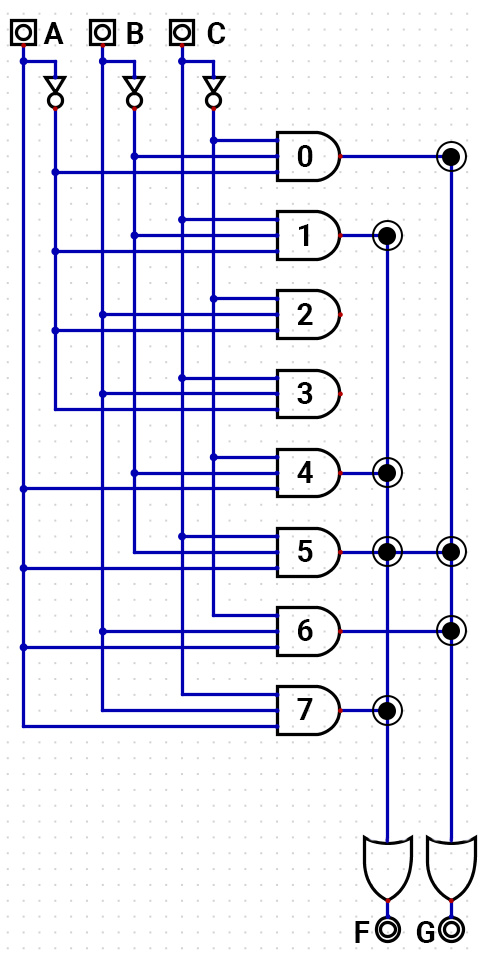
\includegraphics[scale=0.3]{HW4_q3.png}
    \end{center}

    b. Implement both function using as many 2:4 decoders chips (with a single active 
    lowenable) and any other logic gates needed

    \textbf{Solution:}

    \begin{center}
        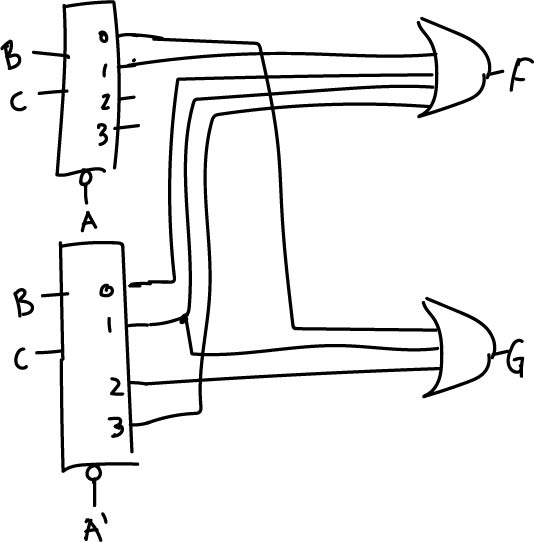
\includegraphics[scale=.35]{HW4_q3_b.jpg}
    \end{center}

    %###################################################################################

    \section*{Problem 4}

    We have a new type of flip flop with inputs A and B. If A = 0,
    then $\text{Q}^+$ = B’ + Q If A = 1, then $\text{Q}^+$ = (AB)’.

    a. Show the state diagram for this flip flop.

    \textbf{Solution:}

    \begin{center}
        \begin{tabular} {c|}
            A  \\
            \hline
            \\
            \\
            0 \\
            \\
            \hline
            \\
            \\
            1 \\
            \\
        \end{tabular}
        \begin{tabular} {cc|c}
            Q & $\text{Q}^+$ & B \\
            \hline
            0 & 0 & 1 \\
            0 & 1 & 0 \\
            1 & 0 & 0 \\
            1 & 1 & 1 \\
            \hline
            0 & 0 & 0 \\
            0 & 1 & 1 \\
            1 & 0 & 0 \\
            1 & 1 & 1 \\
        \end{tabular}
    \end{center}

    \begin{center}
        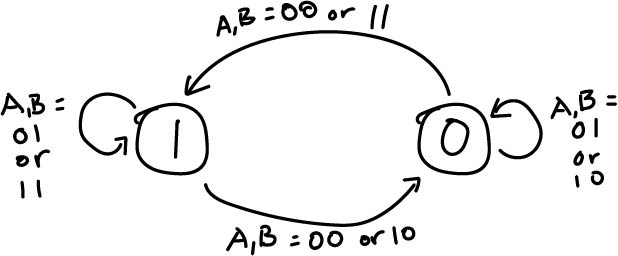
\includegraphics[scale=.35]{HW4_q4.jpg}
    \end{center}

    b. Write a single equation for Q+ in terms of A, B and Q.

    \textbf{Solution:}

    \begin{center}
        \begin{tabular} {cc|cccc}
            & BQ & &&& \\
            A && 00 & 01 & 11 & 10 \\
            \hline
            & 0 & 1 & 0 & 1 & 0 \\
            & 1 & 0 & 1 & 1 & 0 \\
        \end{tabular}
    \end{center}

    $\boxed{\text{Q}^+ = \text{Q(A+B)+A'B'Q'}}$


    %###################################################################################

    \section*{Problem 5}

    Answer the following short answer questions:

    a. Why is a NOT inverter logic gate faster than an open-collector buffer gate?

    \begin{enumerate}[label={\bfseries Solution:}, leftmargin=*]
        \item An open-collector buffer gate consists of two transitors. This, by default,
        would mean that the NOT inverter logic gate is faster than an open-collector
        buffer gate since a NOT inverter gate only contains one transitor.
    \end{enumerate}

    b. What happens when a tri-state buffer has an enable input equal to 0?

    \begin{enumerate}[label={\bfseries Solution:}, leftmargin=*]
        \item When the tri-state buffer has an enable input equal to 0, the buffer behaves as an open
        circuit -- the output is no longer connect to anything. This is called the High-Impedance
        state (Hi-Z).
    \end{enumerate}

    c. A latch and a flip flop differ in what way?

    \begin{enumerate}[label={\bfseries Solution:}, leftmargin=*]
        \item Latches are asynchronous -- the outputs changes soon after the input changes --
        however, most appliances and eletronics operate with an internal clock signal. And 
        so the flip-flop is a synchronout version of the latch meaning it incorporates a
        clock signal so that the outputs changes simultaneously according to the clock.
    \end{enumerate}

    %###################################################################################

    \section*{Problem 6}

    For the input D show below, show the D-latch output (Q) assuming the latch is 
    activated when the enable signal is high.

    \begin{center}
        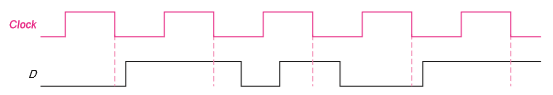
\includegraphics[width=\linewidth]{HW4_q6.png}
    \end{center}

    \textbf{Solution:}

    \begin{center}
        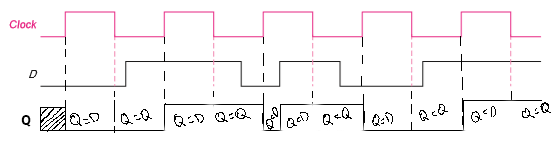
\includegraphics[width=\linewidth]{HW4_q6_s.png}
    \end{center}

    %###################################################################################

    \section*{Problem 7}

    Create the schematic for a new flip flop with the behavior defined by the function 
    below. Use a single D flip flop (positive edge triggered), a single 2:1 multiplexer, 
    and any complemented or uncomplemented variables or additional logic gates needed.

    \[Q^+(x,y,Q)=(Q'+x)+(y'Q')\]

    \textbf{Solution:}

    \begin{center}
        \begin{tabular} {ccc|c}
            x & y & Q & $\text{Q}^+$ \\
            \hline
            0 & 0 & 0 & 1 \\
            0 & 0 & 1 & 0 \\
            0 & 1 & 0 & 1 \\
            0 & 1 & 1 & 0 \\
            1 & 0 & 0 & 1 \\
            1 & 0 & 1 & 1 \\
            1 & 1 & 0 & 1 \\
            1 & 1 & 1 & 1 \\
        \end{tabular}
    \end{center}

    \begin{center}
        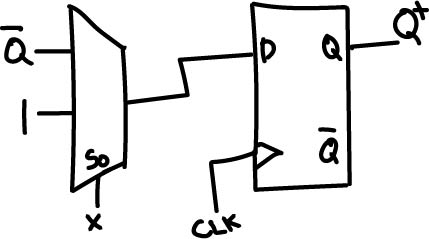
\includegraphics[scale=0.5]{HW4_q7.jpg}
    \end{center}

    %###################################################################################

    \section*{Problem 8}

    For the input shown below, show the flip flop outputs assuming a negative edge trigger.

    \begin{center}
        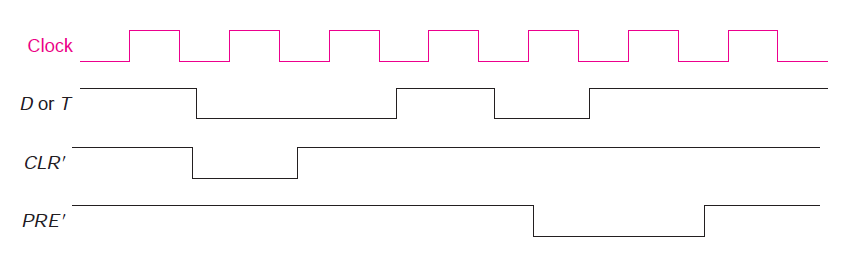
\includegraphics[width=\linewidth]{HW4_q8.png}
    \end{center}

    a. Assume that the flip flop is a T flip flop with only an active low clear (ignore the 
    PRE’ input).

    \textbf{Solution:}

    \begin{center}
        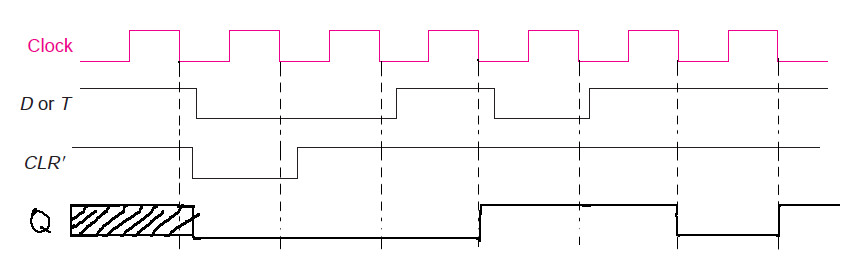
\includegraphics[width=\linewidth]{HW4_q8.1.png}
    \end{center}

    b. Assume that the flip flop is a D flip flop with both an active low clear and active 
    low preset.

    \textbf{Solution:}

    \begin{center}
        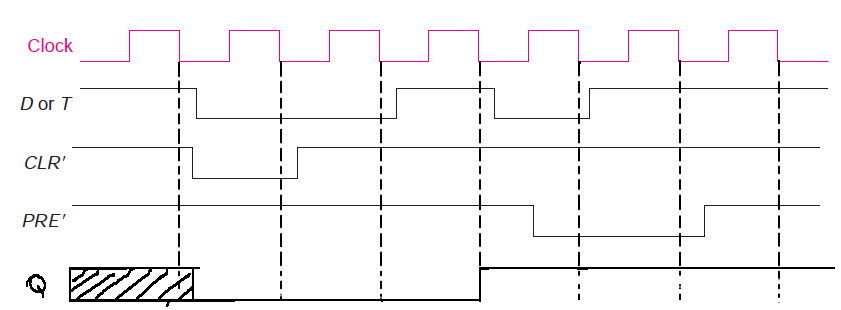
\includegraphics[width=\linewidth]{HW4_q8.2.png}
    \end{center}

    %###################################################################################

    \section*{Problem 9}

    For the following JK flip flop, complete each timing diagram. First, assume the CLR’ 
    and PRE’ are inactive (1). Then use the values shown.

    \begin{center}
        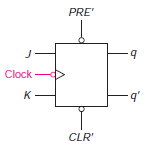
\includegraphics[scale=0.75]{HW4_q9.1.png}
    \end{center}

    \begin{center}
        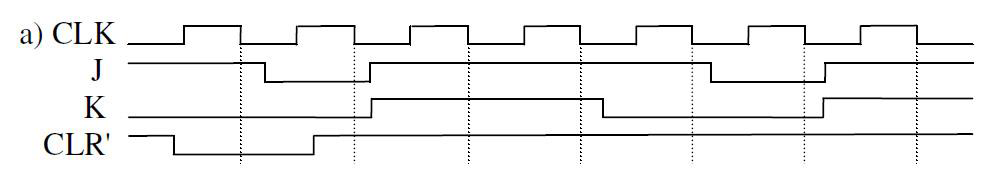
\includegraphics[width=\linewidth]{HW4_q9.2.png}
    \end{center}

    \textbf{Solution:}

    \begin{center}
        \begin{tabular} {cc|c}
            J & K & $\text{Q}^+$ \\
            \hline
            0 & 0 & Q \\
            0 & 1 & 0 \\
            1 & 0 & 1 \\
            1 & 1 & $\overline{\text{Q}}$ \\
        \end{tabular}
    \end{center}

    \begin{center}
        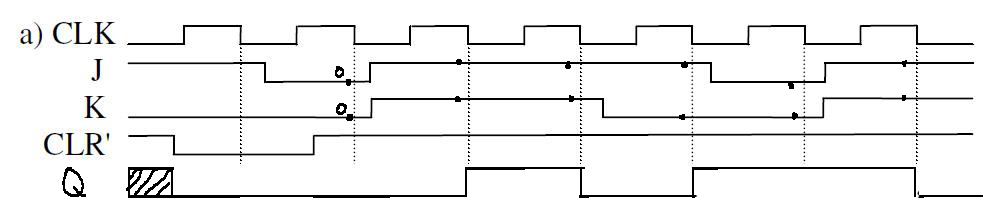
\includegraphics[width=\linewidth]{HW4_q9.2.1.png}
    \end{center}

    \noindent\rule{\textwidth}{0.8pt}

    \begin{center}
        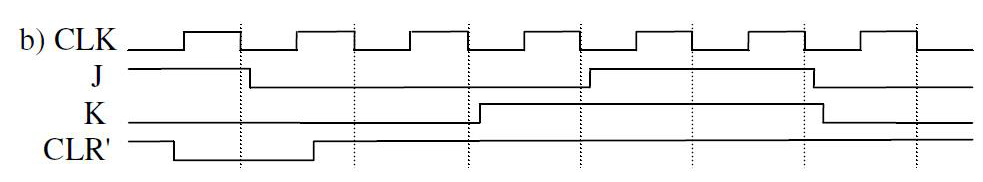
\includegraphics[width=\linewidth]{HW4_q9.3.png}
    \end{center}

    \textbf{Solution:}

    \begin{center}
        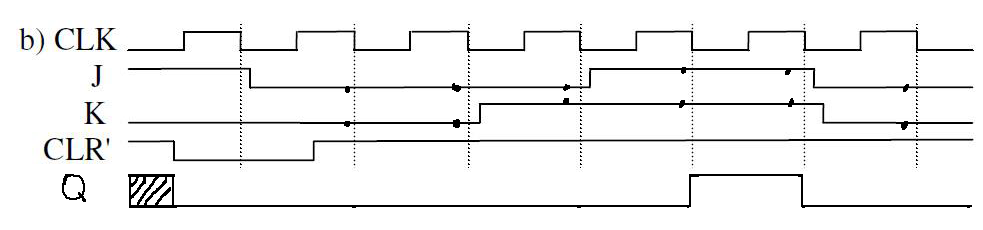
\includegraphics[width=\linewidth]{HW4_q9.3.1.png}
    \end{center}

    \noindent\rule{\textwidth}{0.8pt}

    \begin{center}
        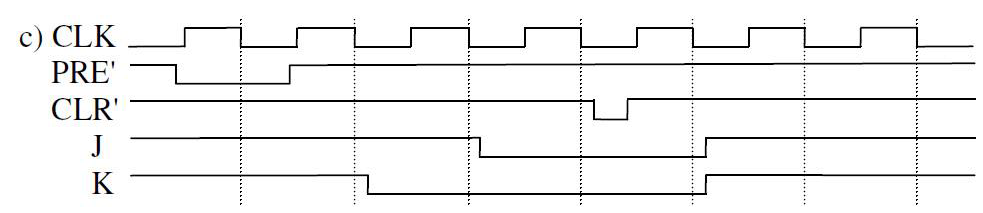
\includegraphics[width=\linewidth]{HW4_q9.4.png}
    \end{center}

    \textbf{Solution:}

    \begin{center}
        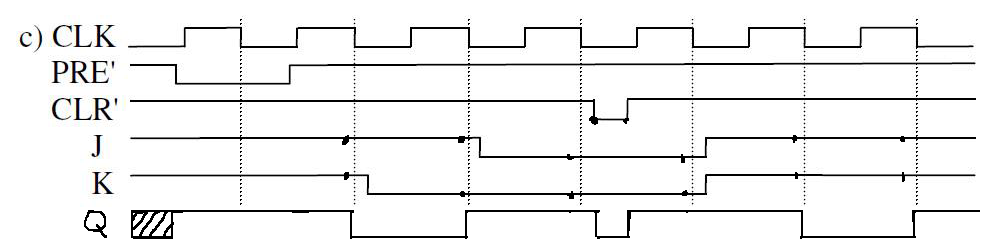
\includegraphics[width=\linewidth]{HW4_q9.4.1.png}
    \end{center}


    %###################################################################################

    \section*{Problem 10}

    For the following circuit, complete the timing diagram assuming negative edge 
    triggering. Include a timing graph for both IN and Q in relation to x. Assume the 
    flip flop is a D flip flop. Assume the flip flop starts at 0.

    \begin{center}
        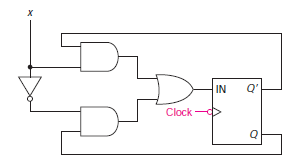
\includegraphics[scale=0.75]{HW4_q10.1.png}
    \end{center}

    \begin{center}
        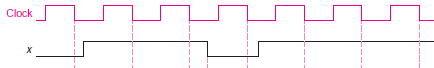
\includegraphics[width=\linewidth]{HW4_q10.2.png}
    \end{center}

    \textbf{Solution:}

    IN equation: $\overline{\text{Q}}\text{x+Q}\overline{\text{x}}$

    \begin{center}
        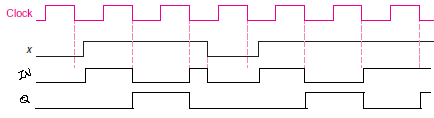
\includegraphics[width=\linewidth]{HW4_q10.2.1.png}
    \end{center}

    %###################################################################################

    \section*{Problem 11}

    For the following circuit, complete the timing diagram for the state of each flip flop 
    and the output, where shown. All flip flops are negative-edge triggered. Assume each 
    flip flop starts at 0.

    \begin{center}
        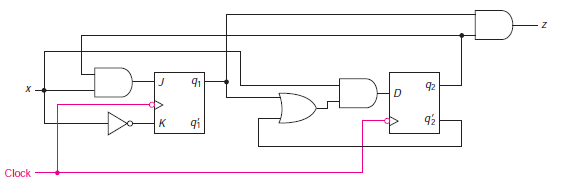
\includegraphics[width=\linewidth]{HW4_q11.1.png}
    \end{center}

    \begin{center}
        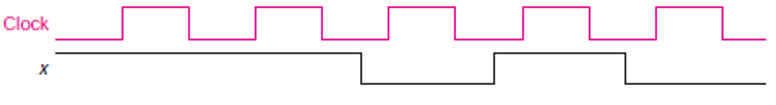
\includegraphics[width=\linewidth]{HW4_q11.2.png}
    \end{center}

    \textbf{Solution:}

    \begin{center}
        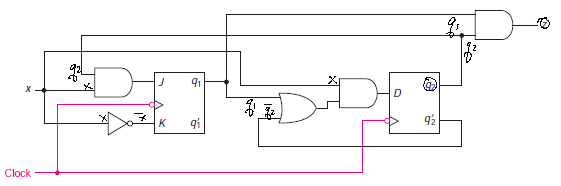
\includegraphics[width=\linewidth]{HW4_q11.1.1.png}
    \end{center}

    J = x$\text{q}_2$
    \quad\quad
    K = $\overline{\text{x}}$
    \quad\quad
    D = x($\text{q}_1+\overline{\text{q}}_2)$
    \quad\quad
    Z = $\text{q}_1\text{q}_2$

    \begin{center}
        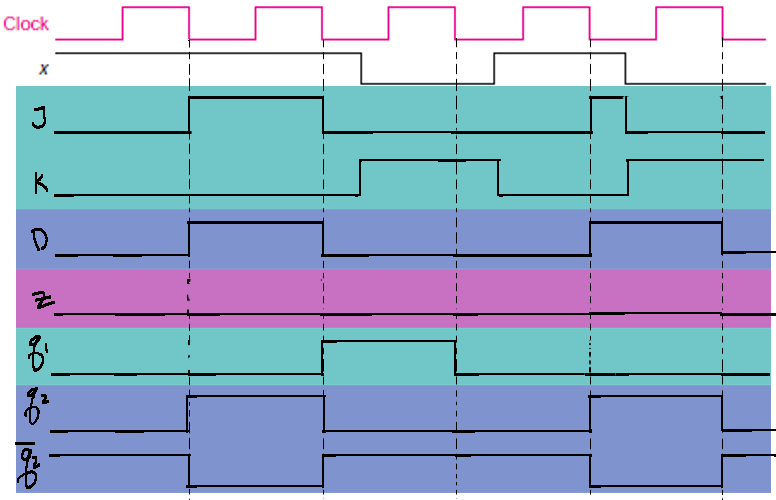
\includegraphics[width=\linewidth]{HW4_q11.2.1.png}
    \end{center}

\end{document}